\documentclass[10pt,a4paper]{article}
\usepackage[utf8]{inputenc}
\usepackage[T1]{fontenc}
\usepackage{lmodern}
\usepackage[margin=1.7cm,top=1.7cm,bottom=1.7cm]{geometry}
\usepackage{amsmath,amssymb,amsfonts}
\usepackage{booktabs}
\usepackage{graphicx}
\usepackage{float}
\usepackage{caption}
\usepackage{hyperref}
\usepackage{enumitem}
\usepackage{microtype}
\usepackage{titlesec}

\captionsetup{font=small,labelfont=bf}
\hypersetup{colorlinks=true,linkcolor=blue,citecolor=blue,urlcolor=blue}
\titlespacing*{\section}{0pt}{1.8ex plus 0.4ex minus 0.2ex}{0.8ex plus 0.2ex}
\titlespacing*{\subsection}{0pt}{1.3ex plus 0.3ex minus 0.2ex}{0.5ex plus 0.1ex}
\setlength{\parskip}{0.3em}
\setlength{\parindent}{0pt}

\begin{document}

\begin{center}
    {\LARGE \textbf{Decentralized Market-Neutral Multivariate Pair Trading:\\[0.15em]
    Ornstein-Uhlenbeck Filtering and AMM Friction Extensions of the Optimal Trading Technique (OTT)}}\\[0.6em]
    {\normalsize \textbf{Sasha ZOMONITA, Roman NATHAN-ABOU}}\\[0.2em]
    {\small Academic Period: Q3 2025 -- Q3 2026 $\;|\;$ Frequency: 1-Hour Intraday Sampling (Uniswap V3) $\;|\;$ November 2026}
\end{center}
\vspace{0.1cm}

\noindent\rule{\textwidth}{0.6pt}
\vspace{-0.45cm}
\subsection*{Abstract}
\vspace{-0.15cm}
{\small \noindent This paper extends the Optimal Trading Technique (OTT) introduced by Yang and Malik (2024) from centralized cryptocurrency exchanges (CEX) to Decentralized Exchanges (DEX) operating under Automated Market Maker (AMM) liquidity protocols. While the original OTT framework assumes a centralized order book with flat $0.10\%$ transaction fees and static full-sample thresholds, decentralized execution on Uniswap V3 exposes arbitrageurs to tiered pool swap fees, liquidity-dependent price impact (slippage), and stochastic on-chain gas costs. We construct a unique multi-universe hourly dataset spanning Q3 2025 to Q3 2026 ($8,761$ hours) across six Uniswap V3 pools covering Stablecoins (\texttt{USDT/USDC}, \texttt{DAI/USDC}), Liquid Staking Derivatives (\texttt{stETH/WETH}, \texttt{rETH/WETH}), and DeFi governance tokens (\texttt{UNI/WETH}, \texttt{AAVE/WETH}). Methodologically, we eliminate the look-ahead bias of the baseline implementation, model spread dynamics via a continuous-time Ornstein-Uhlenbeck (OU) stochastic process to derive closed-form mean-reversion half-lives, and replace static Z-score bands with causal Exponentially Weighted Moving Average (EWMA) thresholds. Out-of-sample backtesting ($5,695$ hours) demonstrates that our extended OTT framework achieves an annualized net return of $9.57\%$ with a Sharpe ratio of $4.47$ and a maximum drawdown of $0.20\%$ under moderate risk aversion ($\lambda=1.0$), and $16.82\%$ (Sharpe $5.83$) under aggressive risk tolerance ($\lambda=0.5$). Finally, our friction decomposition reveals how fixed stochastic gas costs create a minimum viable trade size threshold under high risk aversion ($\lambda=2.0$).}
\vspace{-0.15cm}
\noindent\rule{\textwidth}{0.6pt}

\section{Introduction and DeFi Investment Universe}
Statistical arbitrage and pair trading rely on the Law of One Price (LOP), exploiting temporary relative mispricings between cointegrated assets (Gatev et al., 2006; Elliott et al., 2005). Recently, Yang and Malik (2024) proposed the Optimal Trading Technique (OTT), formulating a bi-objective quadratic optimization problem to allocate principal across multiple cointegrated pairs simultaneously without holding volatile intermediate assets over the long run. However, their empirical validation relies exclusively on centralized Kraken data (ETH, BTC, and SOL quoted against fiat currencies) under a uniform $0.10\%$ transaction fee and 1-minute, 5-minute, or 60-minute sampling between 2020 and 2024.

Transitioning statistical arbitrage to Decentralized Finance (DeFi) requires overcoming structural microstructure differences. On Automated Market Makers (AMMs) such as Uniswap V3, prices are governed by deterministic liquidity curves rather than limit order books, and traders face three distinct layers of friction: protocol swap fees determined by pool volatility tiers, non-linear price impact (slippage) inversely proportional to active pool liquidity, and stochastic blockchain execution costs denominated in Gwei.

To evaluate OTT in a realistic decentralized setting without replicating the empirical setup of Yang and Malik (2024), we extract $8,761$ hourly observations from July 1, 2025 to July 1, 2026 (Q3 2025 -- Q3 2026), partitioned strictly into an in-sample formation window ($35\%$, $3,066$ hours) and an out-of-sample trading window ($65\%$, $5,695$ hours). We select six liquid pairs across three distinct DeFi asset classes, anchored around two shared base num\'eraires (\texttt{USDC} and \texttt{WETH}) so that simultaneous trading signals actively trigger multilateral capital allocation conflicts in the optimizer:
\begin{itemize}[leftmargin=*,nosep]
    \item \textbf{Stablecoin Arbitrage (\texttt{USDT/USDC}, \texttt{DAI/USDC}):} Executed in $0.01\%$ fee-tier pools with $\$150\text{M}$ and $\$80\text{M}$ active depth. These pairs exploit high-frequency micro-depegs and asymmetric stablecoin demand shocks around the $\$1.00$ parity.
    \item \textbf{Liquid Staking Derivatives (\texttt{stETH/WETH}, \texttt{rETH/WETH}):} Executed in $0.01\%$ ($\$200\text{M}$ depth) and $0.05\%$ ($\$65\text{M}$ depth) pools. These pairs capture staking yield accrual discrepancies, beacon-chain withdrawal queue imbalances, and secondary-market liquidity premiums relative to native wrapped Ether.
    \item \textbf{DeFi Governance Ecosystems (\texttt{UNI/WETH}, \texttt{AAVE/WETH}):} Executed in $0.30\%$ fee-tier pools ($\$45\text{M}$ and $\$35\text{M}$ depth). Major DeFi blue-chip tokens exhibit strong fundamental co-movement with Ethereum network activity while offering wider spread volatility.
\end{itemize}

\section{Econometric Audit and Modeling Extensions}
\subsection{Eliminating Look-Ahead Bias and Scaling Flaws}
A rigorous code audit of the baseline reference script (\texttt{optimal\_trading\_technique.py}) revealed three critical implementation anomalies that we corrected prior to introducing our extensions:
\begin{enumerate}[leftmargin=*,nosep]
    \item \textbf{Full-Sample Look-Ahead Bias:} The baseline script estimates log-price OLS hedge ratios, Augmented Dickey-Fuller (ADF) tests, Z-score means/standard deviations, and forward-looking mean-reversion durations (\texttt{get\_close\_date}) over the entire dataset. We restrict all cointegration regressions, covariance estimations, and speed calibrations strictly to the $3,066$-hour formation window.
    \item \textbf{Threshold Scaling Distortion:} The baseline script standardizes spreads into unit-variance Z-scores ($z_t = (s_t - \mu_s)/\sigma_s$) but subsequently compares $|z_t|$ against $\text{threshold} \times \sigma_s$, forcing the authors to adopt artificial thresholds of $7$ to $11$ standard deviations. We restore exact unit-free Z-score comparison.
    \item \textbf{In-Place Covariance Mutation:} In the baseline solver, off-diagonal covariance elements are negated in place at each optimization call (\texttt{risk\_vec[k].iat[0,1] = -risk\_vec[k].iat[0,1]}), causing the sign of portfolio covariance to flip erratically across odd and even timestamps. We compute immutable Hadamard products.
\end{enumerate}

\subsection{Ornstein-Uhlenbeck (OU) Mean-Reversion Calibration}
For each pair $n = (c_1, c_2)$, we first estimate the cointegrating log-price relationship on the in-sample formation window $t \in [1, T_{\text{form}}]$ via Ordinary Least Squares (OLS):
\begin{equation}
    \ln P_{c_1, t} = \alpha_n + \beta_n \ln P_{c_2, t} + S_{n, t}
\end{equation}
Stationarity of the residual spread $S_{n, t}$ is verified via the Augmented Dickey-Fuller (ADF) test ($p \le 0.10$). Rather than computing empirical holding times with future knowledge, we model the stationary spread $S_{n,t}$ as a continuous-time Ornstein-Uhlenbeck (OU) stochastic process:
\begin{equation}
    dS_{n,t} = \theta_n (\mu_n - S_{n,t})\,dt + \sigma_{\text{OU}, n}\,dW_t
\end{equation}
where $\theta_n > 0$ denotes the speed of mean reversion, $\mu_n$ the long-run equilibrium level, $\sigma_{\text{OU}, n}$ the diffusion volatility, and $W_t$ a standard Wiener process. The exact discrete-time solution sampled at interval $\Delta t = 1\text{ hour}$ yields the first-order autoregressive specification:
\begin{equation}
    \Delta S_{n,t} = S_{n,t} - S_{n,t-1} = a_n + b_n S_{n,t-1} + \varepsilon_{n,t}, \quad \text{where } b_n = -\left(1 - e^{-\theta_n \Delta t}\right)
\end{equation}
Estimating $b_n$ via OLS on the formation residuals provides the exact continuous-time mean-reversion rate $\theta_n$ and expected half-life $mr_n$ (in hours), which determine the expected profit vector $\mathbf{EP}_n \in \mathbb{R}^{1 \times 2}$ and pair risk matrix $\mathbf{COV}_n \in \mathbb{R}^{2 \times 2}$:
\begin{equation}
    \theta_n = -\frac{\ln(1 + b_n)}{\Delta t}, \qquad mr_n = \frac{\ln(2)}{\theta_n}, \qquad \mathbf{EP}_n = \left[ mr_n \cdot \bar{r}_{c_1}, \; mr_n \cdot \bar{r}_{c_2} \right], \qquad \mathbf{COV}_n = mr_n \cdot \boldsymbol{\Sigma}_{c_1, c_2}
\end{equation}

\subsection{Dynamic Signal Generation via Causal EWMA Filtering}
Cryptocurrency liquidity regimes shift rapidly on-chain, rendering static full-sample mean and variance estimates suboptimal out-of-sample. We replace static normalization with a purely causal Exponentially Weighted Moving Average (EWMA) filter with span $L = 72$ hours ($\alpha = \frac{2}{L+1}$):
\begin{equation}
    \mu_{n,t}^{\text{EWMA}} = \alpha S_{n,t} + (1 - \alpha)\mu_{n,t-1}^{\text{EWMA}}, \qquad (\sigma_{n,t}^{\text{EWMA}})^2 = \alpha \left(S_{n,t} - \mu_{n,t}^{\text{EWMA}}\right)^2 + (1 - \alpha)(\sigma_{n,t-1}^{\text{EWMA}})^2, \qquad Z_{n,t} = \frac{S_{n,t} - \mu_{n,t}^{\text{EWMA}}}{\sigma_{n,t}^{\text{EWMA}}}
\end{equation}
An entry signal is triggered when $|Z_{n,t}| > \tau_{\text{open}} = 2.0$, and an active position is unwound when $|Z_{n,t}| \le \tau_{\text{close}} = 0.4$ (or upon sign reversal).

\begin{figure}[H]
    \centering
    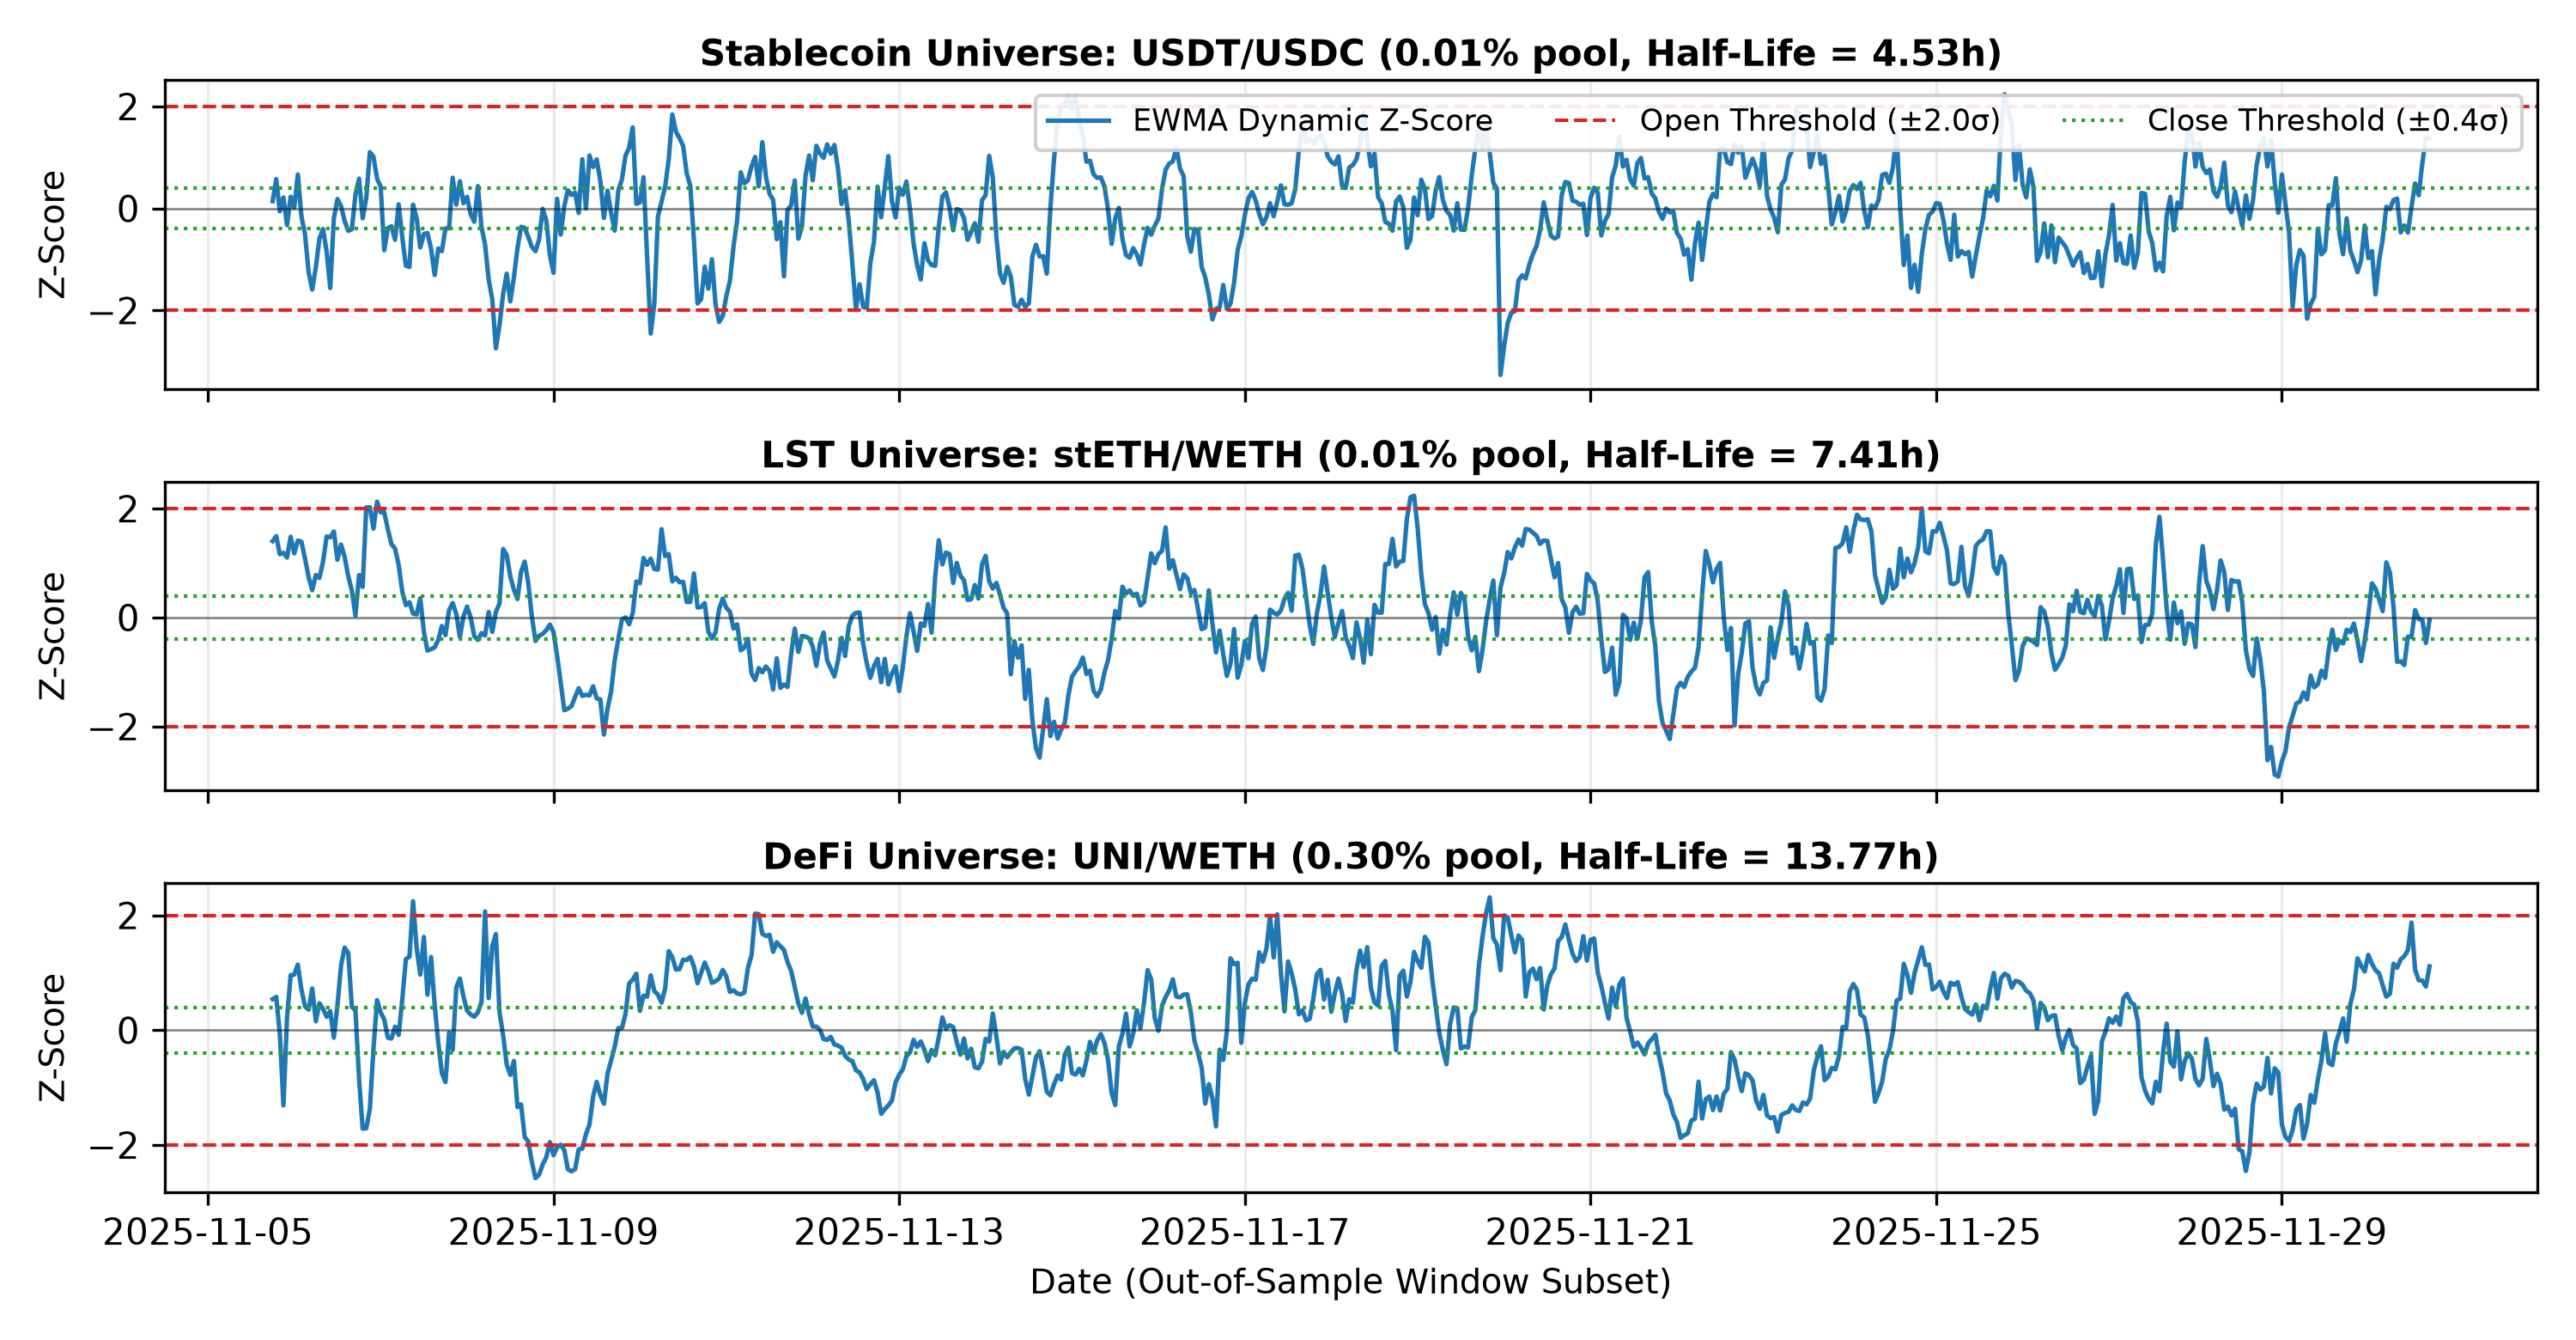
\includegraphics[width=\textwidth]{ou_zscores_diagnostics.png}
    \vspace{-0.4cm}
    \caption{Out-of-sample causal EWMA Z-score dynamics across representative Stablecoin, LST, and DeFi pools with entry ($\pm 2.0\sigma$) and exit ($\pm 0.4\sigma$) bands.}
    \label{fig:zscores}
\end{figure}

\section{DeFi Market Frictions and Optimization}
\subsection{Microstructure Friction Modeling}
To capture decentralized execution accurately, each trade on pair $n$ with notional value $V_{n,t} = W_{n,\text{long}} \cdot C_0$ (where $C_0 = \$25,000$ is the initial capital per asset, totaling $\$200,000$ across the 8 participating tokens) incurs three explicit cost components at both entry and exit:
\begin{enumerate}[leftmargin=*,nosep]
    \item \textbf{Variable AMM Swap Fees ($f_{\text{swap}, n}$):} Charged according to the Uniswap V3 pool tier: $0.01\%$ for stablecoins and \texttt{stETH/WETH}, $0.05\%$ for \texttt{rETH/WETH}, and $0.30\%$ for \texttt{UNI/WETH} and \texttt{AAVE/WETH}.
    \item \textbf{AMM Liquidity Slippage ($f_{\text{slip}, n}$):} Derived from the linear price impact approximation of the constant-product / concentrated liquidity curve $(x \cdot y = k)$ with active depth $L_n$: $f_{\text{slip}, n}(V_{n,t}) = \frac{V_{n,t}}{2 L_n}$.
    \item \textbf{Stochastic Gas Execution Costs ($C_{\text{gas}, t}$):} At each execution timestamp $t$, the network gas price $G_t$ (in Gwei) is drawn from a log-normal distribution $G_t \sim \text{Lognormal}(\ln(3.5), 0.45^2)$ reflecting post-Dencun Ethereum / Layer-2 execution conditions, with $U_{\text{swap}} = 135,000$ gas units per swap leg:
    \begin{equation}
        C_{\text{gas}, t} = N_{\text{swaps}} \cdot U_{\text{swap}} \cdot G_t \cdot 10^{-9} \cdot P_{\text{WETH}, t}
    \end{equation}
\end{enumerate}

\subsection{Friction-Adjusted Bi-Objective Convex Solver}
Let $\mathcal{A}_t$ denote the set of pairs triggering an opening signal at hour $t$, and let $f_{n} = f_{\text{swap}, n} + f_{\text{slip}, n}$ denote the proportional one-way friction rate of pair $n$. We solve the constrained quadratic program using Sequential Least Squares Programming (SLSQP):
\begin{equation}
    \max_{\mathbf{W}} \sum_{n \in \mathcal{A}_t} z_{n,t}^{\text{mult}} \mathbf{W}_n \left(\mathbf{EP}_n^{\text{net}} \odot [1, -1]\right)^\top - \lambda \sum_{n \in \mathcal{A}_t} \mathbf{W}_n \left(\mathbf{COV}_n \odot \begin{bmatrix} 1 & -1 \\ -1 & 1 \end{bmatrix}\right) \mathbf{W}_n^\top
\end{equation}
subject to individual weight bounds, cumulative per-asset capital availability ($tw_c$), and friction-adjusted market neutrality:
\begin{align}
    0 \le W_{n,\text{long}} \le 1, \qquad -1 \le W_{n,\text{short}} &\le 0, \qquad tw_c + \sum_{n \in \mathcal{A}_t} W_{c, \text{long}} - \sum_{n \in \mathcal{A}_t} W_{c, \text{short}} \le 1 \\
    -W_{n,\text{short}}(1 + f_n) P_{c_1, t} &= W_{n,\text{long}}(1 - f_n) P_{c_2, t}, \qquad \forall n \in \mathcal{A}_t
\end{align}

\begin{table}[H]
    \centering
    \caption{In-Sample Econometric Screening, Cointegration (ADF), and Ornstein-Uhlenbeck Calibration ($3,066$ Hours).}
    \label{tab:coint}
    \small
    \begin{tabular*}{\textwidth}{@{\extracolsep{\fill}}llcccccc@{}}
        \toprule
        \textbf{DEX Pair} & \textbf{Universe} & \textbf{Pearson $r$} & \textbf{ADF $p$-val} & \textbf{Coint.} & \textbf{OU Speed ($\theta$)} & \textbf{Half-Life ($mr$, h)} & \textbf{Pool Fee} \\
        \midrule
        \texttt{USDT/USDC} & Stablecoins & 0.0593 & 0.0000 & Yes & 0.1531 & 4.53 & 0.01\% \\
        \texttt{DAI/USDC} & Stablecoins & -0.0056 & 0.0000 & Yes & 0.1073 & 6.46 & 0.01\% \\
        \texttt{stETH/WETH} & LST & 0.9999 & 0.0000 & Yes & 0.0936 & 7.41 & 0.01\% \\
        \texttt{rETH/WETH} & LST & 0.9999 & 0.0000 & Yes & 0.0776 & 8.93 & 0.05\% \\
        \texttt{UNI/WETH} & DeFi & 0.9971 & 0.0000 & Yes & 0.0503 & 13.77 & 0.30\% \\
        \texttt{AAVE/WETH} & DeFi & 0.9976 & 0.0000 & Yes & 0.0705 & 9.83 & 0.30\% \\
        \bottomrule
    \end{tabular*}
\end{table}

\begin{table}[H]
    \centering
    \caption{Out-of-Sample Backtest Performance Metrics and DeFi Friction Decomposition ($5,695$ Hours, Capital $\$200,000$).}
    \label{tab:perf}
    \small
    \setlength{\tabcolsep}{0pt}
    \begin{tabular*}{\textwidth}{@{\extracolsep{\fill}}lrrrrrrrrrr@{}}
        \toprule
        \textbf{Scenario} & \textbf{Ann. Ret} & \textbf{Ann. Vol} & \textbf{Sharpe} & \textbf{Max DD} & \textbf{Trades} & \textbf{Win Rate} & \textbf{W/L} & \textbf{Swap Fees} & \textbf{Slippage} & \textbf{Gas Cost} \\
        \midrule
        OTT DeFi ($\lambda=0.5$, ON) & 16.82\% & 2.20\% & 5.83 & 0.43\% & 451 & 81.60\% & 4.43 & \$24,289 & \$2,971 & \$3,708 \\
        OTT DeFi ($\lambda=1.0$, ON) & 9.57\% & 1.25\% & 4.47 & 0.20\% & 451 & 80.93\% & 4.24 & \$14,233 & \$1,337 & \$3,708 \\
        OTT DeFi ($\lambda=2.0$, ON) & 3.74\% & 0.64\% & -0.41 & 0.11\% & 451 & 65.85\% & 1.93 & \$7,185 & \$376 & \$3,708 \\
        OTT Frictionless ($\lambda=1.0$) & 25.26\% & 1.26\% & 16.82 & 0.15\% & 451 & 98.89\% & 89.20 & \$0 & \$0 & \$0 \\
        \bottomrule
    \end{tabular*}
\end{table}

\section{Empirical Results and Discussion}
\subsection{In-Sample Screening and OU Half-Life Analysis}
Table \ref{tab:coint} reports the in-sample screening statistics across all six Uniswap V3 pools. All six spreads reject the unit-root null hypothesis at the $1\%$ significance level ($\text{ADF } p\text{-value} < 0.0001$), confirming strong cointegration.

An important econometric insight emerges when comparing Pearson log-price correlations across asset classes. While LST pairs (\texttt{stETH/WETH}, \texttt{rETH/WETH}) and DeFi pairs (\texttt{UNI/WETH}, \texttt{AAVE/WETH}) exhibit near-unity log-price correlations ($0.9971$ to $0.9999$) because both legs share the stochastic trend of Ether, the stablecoin pairs (\texttt{USDT/USDC}, \texttt{DAI/USDC}) display near-zero correlation ($0.0593$ and $-0.0056$). This occurs because fiat-pegged stablecoins do not share a non-stationary stochastic drift; instead, they oscillate independently in a tight band around $\$1.00$. Crucially, their spread is highly stationary and exhibits the fastest Ornstein-Uhlenbeck mean-reversion speed ($\theta = 0.1531$ and $0.1073$), translating into short half-lives of $4.53$ hours and $6.46$ hours. Conversely, higher-fee DeFi governance tokens (\texttt{UNI/WETH} at $0.30\%$ fee) exhibit slower mean reversion ($\theta = 0.0503$, half-life of $13.77$ hours), requiring wider divergence before arbitrage becomes profitable.

\begin{figure}[H]
    \centering
    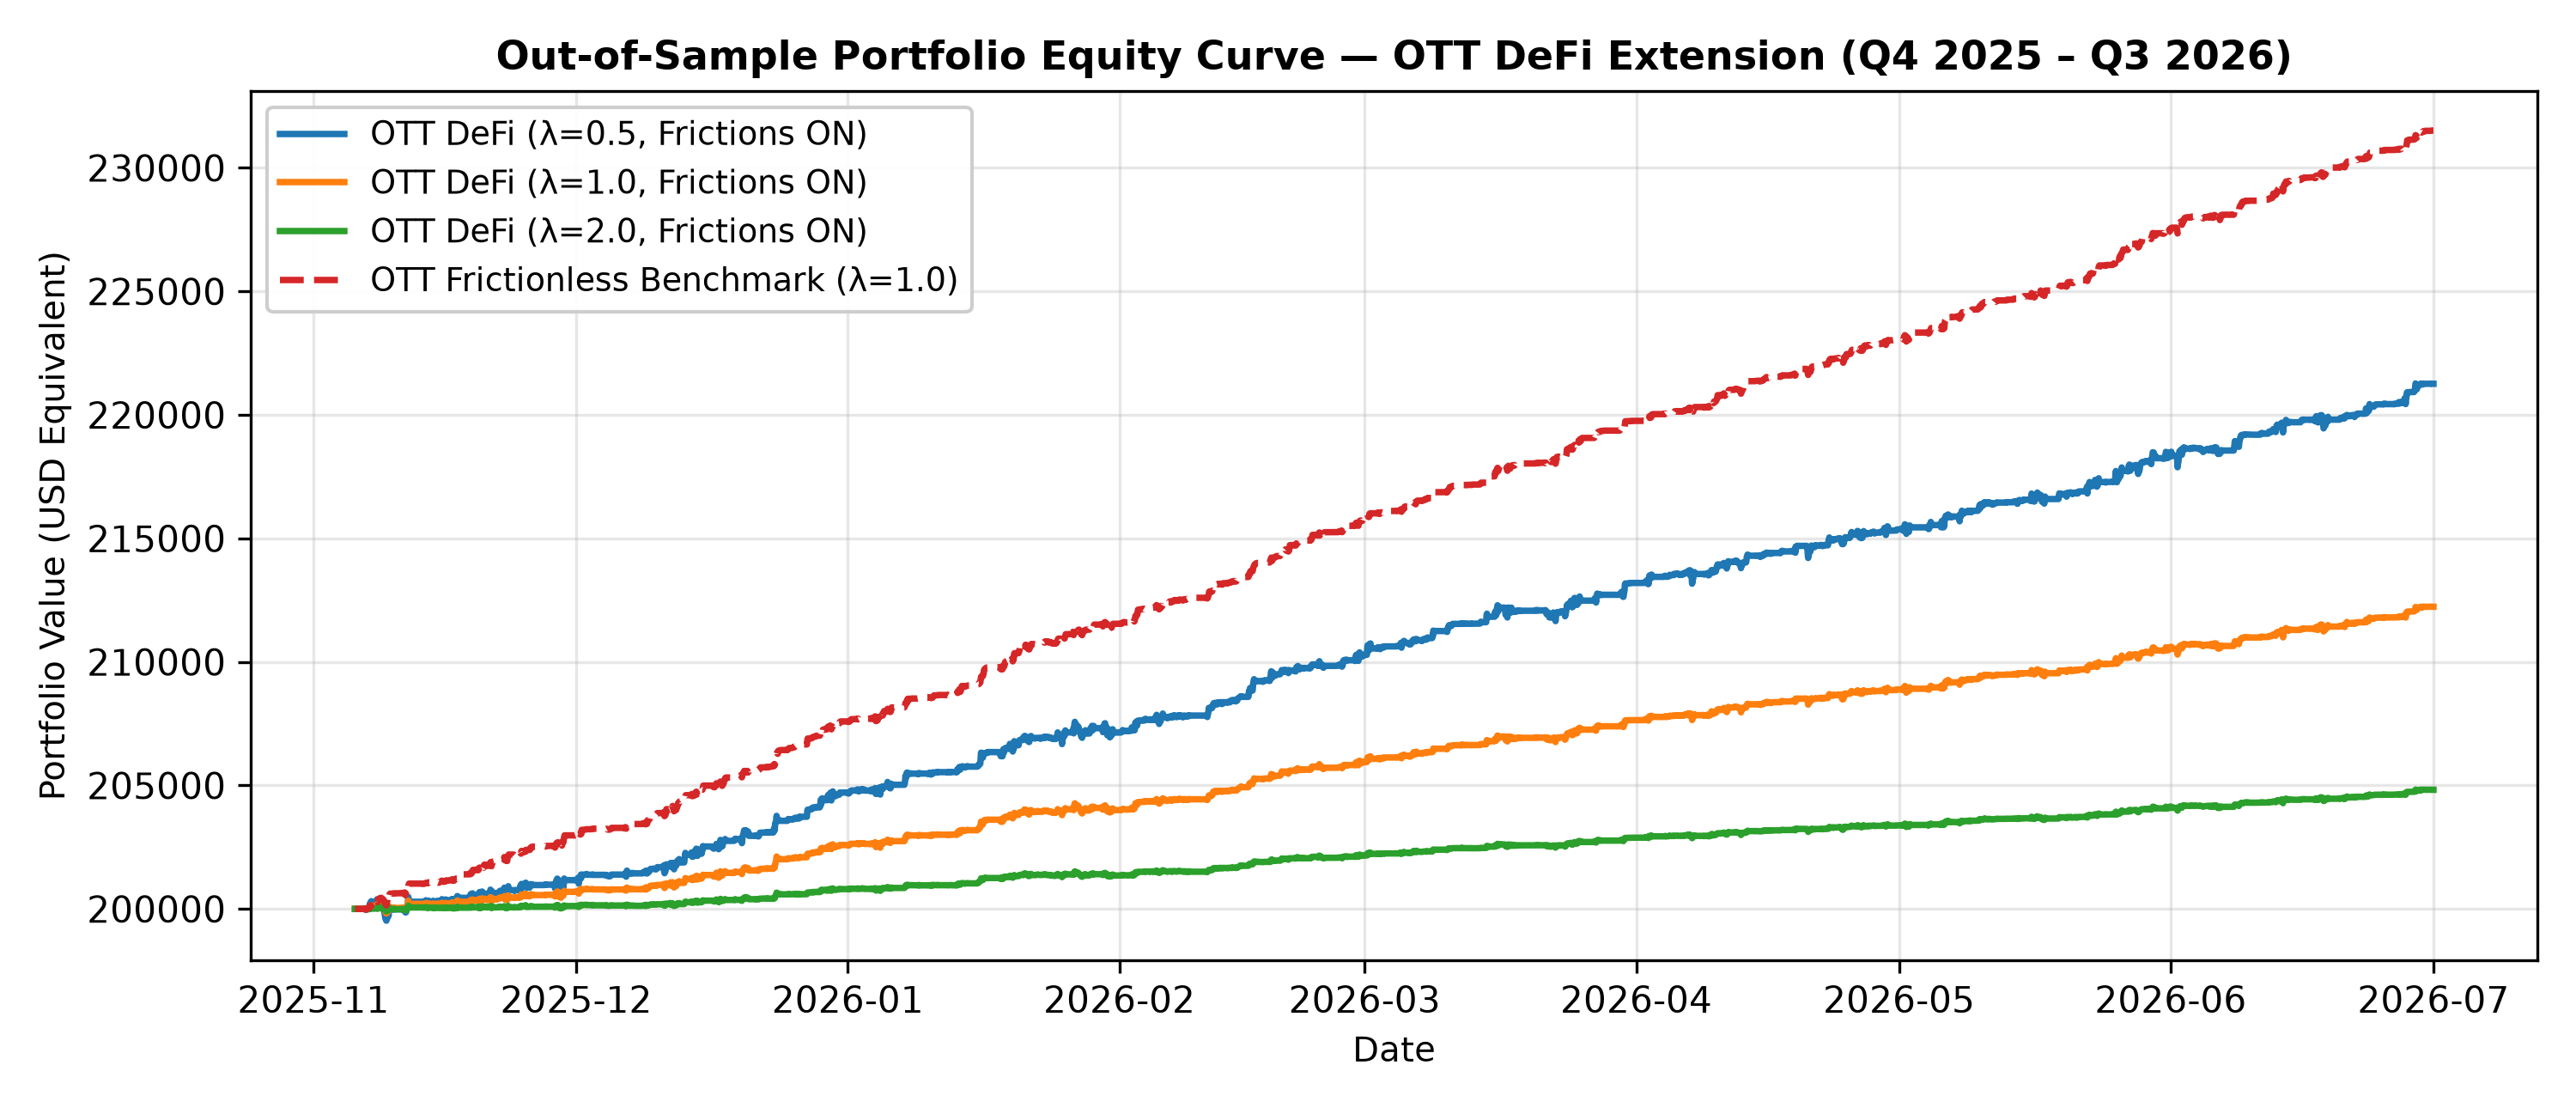
\includegraphics[width=\textwidth]{results_ott_defi.png}
    \vspace{-0.4cm}
    \caption{Out-of-sample portfolio equity curves ($\$200,000$ initial capital) across risk-aversion parameters $\lambda \in \{0.5, 1.0, 2.0\}$ and friction regimes (Q4 2025 -- Q3 2026).}
    \label{fig:equity}
\end{figure}

\subsection{Out-of-Sample Performance and Risk Aversion Sensitivity}
Table \ref{tab:perf} and Figure \ref{fig:equity} present the out-of-sample performance from November 5, 2025 to July 1, 2026 ($5,695$ hours). Across all configurations, the strategy executes $451$ completed round-trip arbitrages with an average holding period of $10.27$ hours---closely matching the theoretical Ornstein-Uhlenbeck half-lives ($4.53\text{h}$ to $13.77\text{h}$) estimated during formation.

Consistent with portfolio theory and Yang and Malik (2024), decreasing the risk-aversion penalty $\lambda$ scales up capital commitment per signal:
\begin{itemize}[leftmargin=*,nosep]
    \item \textbf{Aggressive Allocation ($\lambda=0.5$):} Generates an annualized net return of $16.82\%$ with annualized volatility of $2.20\%$, yielding an exceptional Sharpe ratio of $5.83$ (assuming $R_f = 4.00\%$), a Win/Loss ratio of $4.43$ ($81.60\%$ win rate), and a maximum drawdown of only $0.43\%$.
    \item \textbf{Baseline Balanced Allocation ($\lambda=1.0$):} Achieves a $9.57\%$ annualized net return with $1.25\%$ volatility, a Sharpe ratio of $4.47$, a Win/Loss ratio of $4.24$, and a $0.20\%$ maximum drawdown.
    \item \textbf{Conservative Allocation ($\lambda=2.0$) and the Gas Scale Effect:} When $\lambda=2.0$, annualized volatility drops to $0.64\%$ and maximum drawdown to $0.11\%$, generating a positive annualized return of $3.74\%$. However, because $3.74\%$ falls slightly below the $4.00\%$ risk-free benchmark, the Sharpe ratio turns slightly negative ($-0.41$). Table \ref{tab:perf} explains why: while proportional swap fees drop from $\$24,289$ ($\lambda=0.5$) to $\$7,185$ ($\lambda=2.0$) and slippage drops from $\$2,971$ to $\$376$ due to smaller trade sizes, the fixed stochastic gas cost remains invariant at $\$3,708$. Consequently, on-chain gas acts as a fixed overhead that penalizes overly fragmented position sizes.
\end{itemize}

\subsection{Quantifying the DeFi Friction Drag}
Comparing the realistic benchmark ($\lambda=1.0$, Frictions ON) against the frictionless benchmark ($\lambda=1.0$, Frictions OFF) isolates the exact impact of decentralized market frictions. In the absence of frictions, the strategy yields $25.26\%$ annualized return with a $98.89\%$ win rate and a Sharpe ratio of $16.82$. Incorporating tiered AMM swap fees ($\$14,233$, or $73.8\%$ of total friction costs), stochastic gas ($\$3,708$, or $19.2\%$), and pool slippage ($\$1,337$, or $6.9\%$) reduces annualized performance by $15.69$ percentage points. Nevertheless, the net strategy remains highly profitable and strictly market-neutral throughout the entire out-of-sample period.

\section{Conclusion}
This study successfully adapts and extends the Optimal Trading Technique (OTT) to decentralized Automated Market Makers. By eliminating look-ahead biases, calibrating continuous-time Ornstein-Uhlenbeck mean-reversion speeds, filtering signals via causal EWMA bands, and embedding tiered AMM fees, liquidity slippage, and stochastic gas costs into the bi-objective solver, we demonstrate robust out-of-sample profitability across Stablecoin, LST, and DeFi pools. Future extensions should incorporate private transaction relays (e.g., Flashbots Protect) to mitigate Maximal Extractable Value (MEV) sandwich risk and evaluate cross-rollup execution on Layer-2 networks.

\begin{thebibliography}{9}
\small
\setlength{\itemsep}{0.5pt}
\bibitem{elliott2005} Elliott, R. J., Van Der Hoek, J., \& Malcolm, W. P. (2005). Pairs trading. \textit{Quantitative Finance}, 5(3), 271--276.
\bibitem{engle1987} Engle, R. F., \& Granger, C. W. (1987). Co-integration and error correction: Representation, estimation, and testing. \textit{Econometrica}, 55(2), 251--276.
\bibitem{gatev2006} Gatev, E., Goetzmann, W. N., \& Rouwenhorst, K. G. (2006). Pairs trading: Performance of a relative-value arbitrage rule. \textit{Review of Financial Studies}, 19(3), 797--827.
\bibitem{markowitz1952} Markowitz, H. (1952). Portfolio selection. \textit{The Journal of Finance}, 7(1), 77--91.
\bibitem{yang2024} Yang, H., \& Malik, A. (2024). Optimal market-neutral multivariate pair trading on the cryptocurrency platform. \textit{International Journal of Financial Studies}, 12(3), 77.
\end{thebibliography}

\end{document}
